%!TEX TS-options = -shell-escape
\documentclass[oribibl]{llncs}
\pagestyle{headings} %page numbers
\usepackage{makeidx}  % allows for indexgeneration

\usepackage[utf8]{inputenc}
\usepackage{pdfpages}

% \usepackage[nottoc,numbib]{tocbibind}
% \usepackage[center]{caption}

\usepackage{float}

\usepackage{enumitem}
\usepackage[T1]{fontenc} % Fixed missing font warning for \maketitle
%\usepackage[margin=1.5in]{geometry}
\usepackage{url}
\usepackage[multiple]{footmisc} % DOUBLE FOOTNOTES ACROSS THE SKY
\renewcommand{\footnotemargin}{3.99pt}

% %% to make urls look better in bibliography
% \makeatletter
% \def\url@leostyle{%
%   \@ifundefined{selectfont}{\def\UrlFont{\sf}}{\def\UrlFont{\small\ttfamily}}}
% \makeatother
% %% Now actually use the newly defined style.
% \urlstyle{leo}

\bibliographystyle{plain}



\begin{document}

% insert the table of contents if want, it is not required
% llncs says: "If you are the author of a single contribution you
% normally have no running heads and no table of contents."
% \tableofcontents

\mainmatter              % start of the contributionsmainmatter
\title{Textual Editing of Partial IFC Model}

\author{Nicolai Dahl Blicher-Petersen \and Christian Harrington \and
Thomas Hallier Didriksen \and Sune Alkærsig \and Anders Høst Kjærgaard\\
\email{\{ndbl, cnha, thdi, sual, ahkj\}@itu.dk}}

% Do we want to show our emails?
\institute{IT University of Copenhagen, Rued Langgaards Vej 7, 2300 Copenhagen S, Denmark}


\maketitle              % typeset the title of the contribution

\begin{abstract}
Industry Foundation Classes (IFC) is an ISO standard used for modelling various physical and functional aspects of a building. IFC models are often large and complex, so a key challenge is: how can work be carried out on e.g. plumbing, heating, or electrical wiring independently, without introducing inconsistencies. This paper describes a prototype solution that eases cross-disciplinary work, by allowing model evolution and resolution of inconsistencies on a small subset of a large IFC model. The model-driven methodology is used to achieve a generally applicable and flexible solution, usable in various domains. In this paper we demonstrate an open source prototype handling a common industry problem that specifically makes it possible to edit pipes, walls, and openings in walls.

\keywords{IFC, BIM, EMF, DSL, model-driven development, model transformation, Xtext, Xtend, BIMServer}
\end{abstract}


%!TEX root = ./report.tex

% Slides:
% - General statement introducing the area; You can most likely start with the first paragraph from your project description and evolve it.
% - Explanation of the specific problem and why do we care about the problem.
% - Explanation of your solution, and how it improves on the work by others. Relation to related work can be very brief, given that you have a separate extensive section devoted to this.
%  -A hint on how the solution was evaluated and what was the outcome of this evaluation.
%  -A summary (a “map”) of how the paper is organized.

\pagenumbering{arabic}
\setcounter{page}{1}
\section{Introduction}
Building Information Modeling (BIM) is the process of modelling various physical and functional aspects of a building. Currently, many BIM software products exist. These allow users to model and analyse the many interactions between different parts of a building. Many of these software products use common file formats for modelling buildings, such as Industry Foundation Classes (IFC). This specification improves interoperability between different software packages in different domains, and is integrated into a variety of commercial applications.

In a real-life scenario, engineers usually work on separate parts of a building model using advanced, proprietary, and visual tools such as Revit.\footnote{An overview of Revit products can be found at \url{http://usa.autodesk.com/revit/}} Due to the complexity of most BIM projects, it is desirable to be able to work with aspects of a model such as heating, electrical wiring, or plumbing independently. In this paper, we present a prototype that demonstrates that such editing on a subset of an IFC model is feasible using modern modelling tools from the Eclipse Modeling Framework (EMF).

\subsubsection{Problem}
In particular, we focus on solving a common problem of combining a construction model with a plumbing model in a manageable way. When modelling buildings, the structure of the building and its plumbing installations are modelled separately\,\cite[pp. 19--20]{jorgensen10}. The construction model describes which walls are load-bearing and which walls have openings for installations. Because of this separate modelling, it is possible for plumbing installations to be inconsistent with the construction model. For example, a pipe could intersect a solid wall, without an opening for it to go through. This could result in a situation at the construction site where a planned installation is not possible in reality. This problem has been defined by Kaj A. Jørgensen\,\cite{jorgensen12}, associate professor at Aalborg University, who has substantial domain knowledge, through his work with IT methodologies for building modelling.\footnote{Kaj A. Jørgensen at Aalborg University: \url{http://www.kaj.person.aau.dk/}}

\subsubsection{Solution}
Due to the difficulties mentioned above, it would be desirable if the construction engineer had an easy way to find these collisions and solve them by making an opening or moving the installation\,\cite{jorgensen12}. To facilitate this, we will\ldots
\begin{itemize}
\item Produce an analysis of the subset of IFC used to define pipe installations, and develop a simple, textual domain specific language (DSL), called Pipes, to specify these installations.
\item Develop an Eclipse editor that eases the writing of files with the DSL, including syntax highlighting and autocompletion.
\item Create an update mechanism between the DSL and the IFC model being manipulated, so changes made in the DSL are applied correctly to the model.
\item Interface with a central server for storing, merging and (future) collaboration support. We use BIMServer\footnote{BIMServer Documentation can be found at \url{http://bimserver.org/documentation/}}, which is open source.
\item Present ideas for future BIM projects in relation to the ITU research initiative Energy Futures, based on this project.\footnote{For further information, see \url{http://energyfutures.itu.dk/}}
\end{itemize}

\subsubsection{Workflow}
\label{sec:workflow}
The workflow revolves around a server. We save a construction model and a plumbing model on the BIMServer, which then merges the two. This merged IFC model is retrieved by our client, and the relevant parts are extracted and transformed to the Pipes DSL syntax. An editor for the Pipes DSL is launched, and the user can edit and verify the consistency of its data and structure. Finally, these changes are updated in the merged model and stored server-side. The prototype solution is extensible and constitutes a good starting point for future automation of the workflow and visualisation of the domain.

\paragraph{}
This paper is structured as follows. In Section \ref{sec:background} we provide a background of the problem space, and in Section \ref{sec:problem_analysis_and_requirements} we analyse the problem and list prototype requirements. Section \ref{sec:solution} describes the solution, which we evaluate in Section \ref{sec:evaluation}. In Section \ref{sec:plan_for_future_projects} we suggest ideas for future projects. Section \ref{sec:related_work} lists related work, and we conclude on our findings in Section \ref{sec:conclusion}.

%!TEX root = ./report.tex
\section{Background}
\label{sec:background}
\subsection{Building Information Modeling}
\label{sec:building_information_modeling}
As previously described, BIM is a process that models physical constructions by generating digital representations. The resulting model is a shared knowledge base that can be used in all stages of a building project. BIM extends traditional building design from two-dimensional drawings and three-dimensional physical models, to include aspects such as time, cost, staffing, and design process. This makes BIM very attractive for modern building construction, as it not only eases the communication between the different stakeholders, but also allows for early planning in terms of time and energy consumption.

To support the flexibility required in BIM, this shared knowledge base has to be represented in a format that enables interoperability. And since building projects involve many different contributors from different domains, it has to be adoptable by many different software applications\,\cite{quteprints37725}. Consequently, an interoperability standard is needed.

\subsection{Industry Foundation Classes}
\label{sec:industry_foundation_classes}
IFC is widely used for BIM, and is mandatory for new public buildings in Denmark.\footnote{Regulations for buildings built by the Danish state: \url{https://www.retsinformation.dk/forms/R0710.aspx?id=134884}} Its goal is to facilitate interoperability between different software platforms\,\cite{steel11} and can reduce time spent on building design processes\,\cite{bazjanac99}. It does this through an object-based data model, represented in two file formats. The first is a EXPRESS-based format, IFC-EXPRESS (ISO-10303-21). The other is an XML format, called ifcXML (ISO-10303-28). The EXPRESS-based format is the most widely used due to its relative compact size, while still being readable.

One of the main challenges when working with IFC is that the models often are very large and complex. The meta model contains more than six hundred entities organised in an object-based inheritance hierarchy. Entities can be both tangible elements, such as an IfcWall, but also abstract entities like IfcAxis2Placement3D, describing the location and orientation of another IFC entity. On the highest level of abstraction, IFC defines two categories of elements: rooted and unrooted elements respectively. Unrooted elements do not have an identity and only exist if referred to by other elements. Rooted elements have a unique global identifier (globalId).\footnote{IFC2x3 Final Documentation: \url{http://www.buildingsmart-tech.org/ifc/IFC2x3/TC1/html/index.htm}}

\subsection{Eclipse Modeling Framework and Ecore}
The Eclipse Modeling Framework is a modelling framework and code generation facility for building tools and other applications, based on a structured data model.\footnote{The EMF project page can be found at \url{http://www.eclipse.org/modeling/emf/} and leads to MWE2, Xtext, Xtend, and Xpand resources.} EMF is capable of producing a Java object graph from a model instance described in XMI. For meta modelling, EMF features Ecore. Ecore is a meta modelling language allowing the user to describe and build meta models for their domain. Furthermore, several transformation tools, such as Xtend and Xpand, are associated with EMF. They support work with model transformations. Xtend is a programming language that compiles into Java. It is very well integrated into EMF, and has several language features that are well suited for model-to-model transformations. Xtend is implemented with Xtext, a tool allowing easy creation of DSLs. Xpand is a template language used in model-to-text transformations. EMF also features a workflow system, Modeling Workflow Engine 2 (MWE2), that makes it easy to chain these tools together.

%!TEX root = ./report.tex
\section{Problem Analysis and Requirements}
\label{sec:problem_analysis_and_requirements}
In the following section we will analyse the problem, and discuss a set of requirements for a solution that is capable of editing a partial IFC model within a specific domain. This list should be thought of as a guideline for how one should ideally approach this problem.

\subsection{Problem Analysis}
\label{subsec:problem_analysis}
The separation of the construction and plumbing models makes it difficult to work on objects that are separated but interrelated. We focus on the case of IfcFlowSegments (i.e. a pipe), IfcWallStandardCases (a regular wall) and an IfcOpeningElement (an opening in a regular wall). Jørgensen mentions that a possible solution to the problem is to allow the building service engineer, responsible for the plumbing installations, to create a message with precise information about required openings for the pipes\,\cite{jorgensen12}. This message could then be handed to the construction engineer, so that he can verify that these are properly placed. As such, the primary goal of the solution is to enable the user to work on a subset of the IFC model involving pipes, openings, and walls. In Figure \ref{fig:ifcheirachy}, a graphical representation of this subset is presented.

\begin{figure}[t]
    \centering
        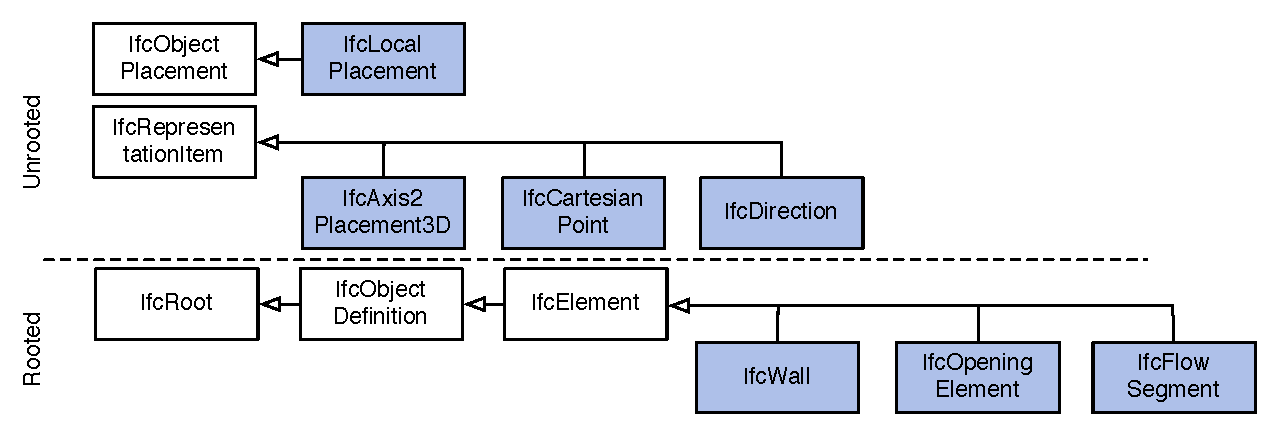
\includegraphics[width=110mm]{images/IfcHeirachy.pdf}
    \caption{A graphical representation of the subset used, excluding relational objects for the sake of simplicity. The concrete classes of the chosen subdomain are highlighted in blue.}
    \label{fig:ifcheirachy}
\end{figure}

\subsection{Requirements}
\label{subsec:requirements}
\subsubsection{R1. Working with a Partial Model}
With the aforementioned complexities and challenges of IFC in mind, a primary focus is to be able to extract a well-specified subset of an IFC model. It is desirable to have an architecture that separates the extraction of a partial model from the rest of the workflow. This component will only extract the IFC elements that we are interested in. This should make the component easier to reuse, and make it easier to verify that the extraction is performed correctly.

Furthermore, a clear domain definition is needed to implement and verify the extraction of the partial model. Achieving this in a concise but generic way is not trivial. An evolving standard for doing this is via Model View Definitions (MVD)\,\cite{nour08}, which allow fine-grained definitions of IFC subsets using XML. The non-profit organisation, buildingSMART, that supports open source BIM software, propagates MVD as their standard.\footnote{buildingSMART, MVD, \url{http://buildingsmart.com/standards/mvd}} Nour discusses this and other challenges when working with partial editing on IFC\,\cite{nour08}. Unfortunately, it was not possible to obtain the product of Nour's project. Even though MVD seems to be a promising approach for extracting IFC subsets, it is outside the scope of this project to develop this functionality ourselves. We found that simply defining a partial model with MVD is in itself a somewhat complex task. Therefore, for the purposes of designing a single experimental DSL with only a few IFC classes, we argue that a more informal definition of the domain is sufficient and will simplify the development process.

\subsubsection{R2. Correct Meta Model}
It is vital for the solution that the IFC meta model is in fact correct. This point may seem obvious at first, but in our experience, finding a correct EMF meta model that reflects the actual IFC standard is difficult. In particular, finding a meta model with a proper serialiser and deserialiser that converts from either IFC-EXPRESS or ifcXML to the corresponding Ecore instance can be difficult. Further, IFC models are not treated consistently across existing BIM software. Thus, one must be aware of inconsistencies\,\cite[p. 4]{quteprints37725}.

\subsubsection{R3. Valid Model Transformations}
An ideal solution would feature model transformations that are verifiable and correct. By verifiable, we mean being able to trace or test that transformations actually occur in the way that we expect. By correct, we mean not corrupting any model structure during a transformation. However, with the complexity of IFC in mind, we allow that some constraints are broken in the IFC model at the end of the transformation. A possible scenario is that in an IFC model, all pipe objects could be referenced by some central element, e.g. for calculation of maintenance costs for these. It would be difficult to require and assert that no such constraints are broken in the general case, and is a problem outside the scope of this project.

\subsubsection{R4. A Simple DSL}
The simple DSL will demonstrate that the editing of partial models is feasible for our own, as well as other, similar subdomains of IFC. The implementation will show how a small, but significant domain can be managed separately from the full IFC model. To support extensibility and reusability, it should be built with widely used tools, like the ones in EMF.  One could imagine that a future solution would have a visual syntax instead of a textual syntax.

\subsubsection{R5. Structural Editing}
It must be possible to use the DSL to add and remove elements. This is required to resemble a real-world scenario, where an element could be missing. The solution must be able to do this for flow segments and openings, without corrupting the IFC model. Structural editing of walls is not needed for the workflow described above, so it may be omitted.

\subsubsection{}
This concludes the list of desirable features, but please note that it is only a core selection, and that many extensions could be added to it. Some of these will be discussed in Section \ref{sec:plan_for_future_projects} as ideas for a future projects.


%!TEX root = ./report.tex
\section{Solution}
\label{sec:solution}
Our prototype combines several open source technologies to attain an extensible solution, with two reusable MWE2 client side workflows at its core. The setup allows the user to edit a subset of IFC in an auto-generated Eclipse editor in between the two workflows. The two building models are stored on a BIMServer for possible merging, version control, and collaboration through use of the client-server design pattern, as this section will explain further. The prototype serves as an open source alternative to similar, proprietary BIM software.

\subsection{IFC Meta Model}
% Our meta model is generated from ifcXML XSD, only handles ifcXML
% BIMServer - tightly coupled, but handles .ifc. Handles references as string
% Jim Steel model. Seems to be better, but we have no deserializer.
\label{subsec:ifc_meta_model}
The prototype uses an IFC meta model that is auto-generated from the XML Schema Definition (XSD) of ifcXML.\footnote{ifcXML XSD: \url{http://buildingsmart-tech.org/ifcXML/IFC2x3/FINAL/IFC2X3.xsd}} This allows utilisation of the XML serialiser and deserialiser provided by EMF, to convert ifcXML to and from its Java representation.  One of the advantages of using these tools is that we do not have to develop any serialisers ourselves. However, generating the meta model from an XSD also means that the client application of the prototype only supports ifcXML, and not  the more widely used IFC-EXPRESS format. Because BIMServer accepts and generates both formats, this is a minor concern. But it means that the client side of the prototype relies on BIMServer for IFC-EXPRESS handling.

Although we chose not to use it, BIMServer also provides a meta model for IFC. This meta model comes with a custom serialiser and deserialiser for IFC-EXPRESS. We found that using this meta model and the provided serialisation tools was undesirable, as it would mean that the client application of the prototype would be completely dependent on the BIMServer. An advantage of using this meta model would be that it resembles the documented IFC specification more closely than the auto-generated meta model (even though both are equally correct). Specifically, the BIMServer meta model includes inverse relationships, which are not represented in the generated meta model, as they are not modelled in ifcXML\,\cite[p. 24]{ifcXMLimpl}.

A third meta model for IFC has been created by Jim Steel, Lecturer at the University of Queensland.\footnote{Jim Steel at the University of Queensland: \url{http://itee.uq.edu.au/~uqjstee8/}}\footnote{Jim Steel's model can be found at \url{http://www.emn.fr/z-info/atlanmod/index.php/Ecore#ifc2x3_0.1}} This meta model seems to model all relationships better than the two aforementioned models, but does not provide a deserialiser to any IFC format. As it is not within the scope of this project to create a deserialiser for such a meta model, it was not used. However, using this meta model could be considered as a future improvement.

\subsection{Pipes DSL}
\label{subsec:pipes_dsl}

\begin{figure}[t]
    \centering
        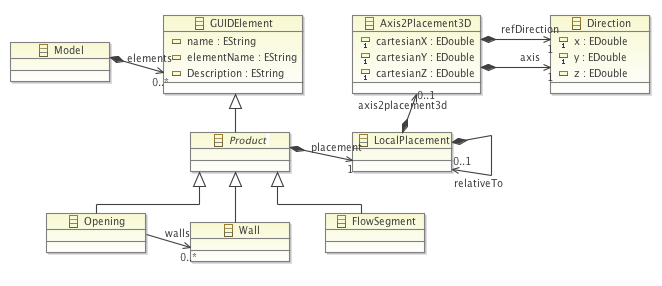
\includegraphics[width=110mm]{images/PipesEcoreModel.png}
    \caption{Pipes DSL Ecore meta model.}
    \label{fig:pipes_dsl_ecore_model}
\end{figure}

\begin{figure}[t]
    \centering
        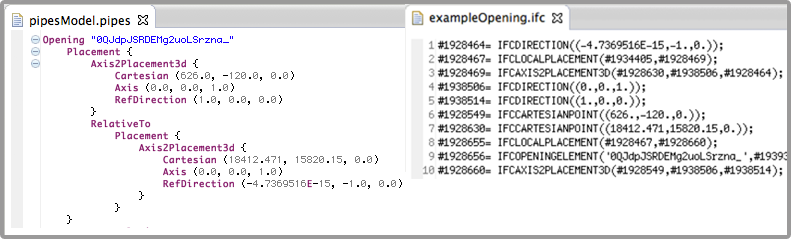
\includegraphics[width=120mm]{images/pipesAndExpressExample.png}
    \caption{A comparison of an opening specification in the Pipes DSL (left) and the IFC-EXPRESS format (right) with placement references and metadata.}
    \label{fig:pipes_express_comparison}
\end{figure}

The simple Pipes DSL serves as the front-end of the prototype. Figure \ref{fig:pipes_dsl_ecore_model} shows the Ecore meta model that the DSL is built upon. Compared to Figure \ref{fig:ifcheirachy}, all the critical elements of the domain are still present, but the inheritance hierarchy has been greatly simplified. As shown, Opening, Wall, and FlowSegment are top level elements, each with a physical location specified by the LocalPlacement reference. Figure \ref{fig:pipes_express_comparison} depicts an example of an opening as it is defined in the Pipes DSL in an uncluttered and manageable way, compared to the IFC-EXPRESS format. The textual syntax has been created from the Pipes DSL meta model using Xtext, which also provides an editor with syntax highlighting and autocompletion. The editor is launched as an Eclipse instance.

\subsection{BIMServer}
The overall workflow of the final product is shown in Figure \ref{fig:overall_product_workflow}. As described in J\o rgensen's workflow document\,\cite{jorgensen12}, a construction model and a plumbing model are combined into a single model that needs to be verified. Openings need to be present where the plumbing model defines pipes are to be installed. The user merges these models on BIMServer as the first step of the workflow. When the models have been merged, the client application can retrieve the merged model as ifcXML. The user is now allowed to edit and add elements to the subset of the model on the client side, before sending the building model back to the BIMServer as ifcXML.

Note that the prototype solution does not take concurrent editing by multiple clients into account, although BIMServer does support version control and change notifications for this exact purpose.

\begin{figure}[t]
    \centering
        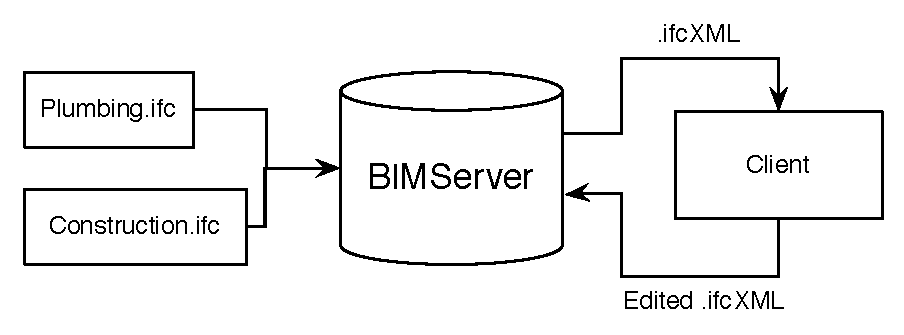
\includegraphics[width=70mm]{images/CompleteWorkflow.pdf}
    \caption{Overall product workflow starting with a merge of two models. The user can edit a subset of the model through the client-side application.}
    \label{fig:overall_product_workflow}
\end{figure}

\subsection{Client Application of the Prototype}
The client side of the prototype is implemented as two MWE2 workflows and a textual editor for the Pipes DSL. The workflows, called IFC2Pipes and Pipes2IFC, invoke a series of workflow components, implemented in Xtend. The IFC2Pipes workflow executes the transformations from IFC to the Pipes DSL, after which the textual editor can be used to modify the Pipes DSL model. When the editing is complete, the Pipes2IFC workflow is run to update the IFC model, based on the changes in the Pipes DSL model.

\begin{figure}[H]
    \centering
        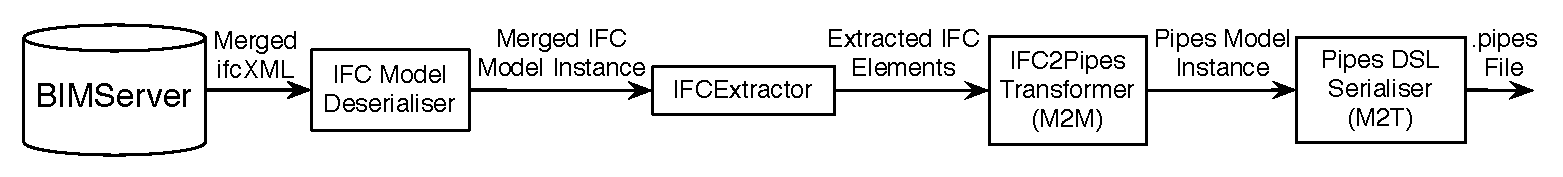
\includegraphics[width=116mm]{images/IFC2Pipes.pdf}
    \caption{IFC2Pipes workflow. Processes ifcXML from BIMServer and outputs a .pipes file, loadable in the Pipes DSL editor.}
    \label{fig:IFC2PipesWorkflow}
\end{figure}
\subsubsection{IFC2Pipes}
Figure \ref{fig:IFC2PipesWorkflow} illustrates the first workflow. The newest revision of the IFC model is downloaded from BIMServer as ifcXML, and cached on disk. This is deserialised by the deserialiser. After the model has been loaded into memory, the relevant elements (see Section \ref{subsec:requirements}) are extracted by a workflow component, IFCExtractor. These elements are passed to the IFC2PipesTransformer component, which creates a Pipes DSL model based on the extracted elements. This is done by creating a Pipes DSL model equivalent for each extracted element, preserving the global ID. Finally, using an Xpand template, text conforming to the concrete syntax for Pipes DSL is generated, and serialised to a file on disk.

\begin{figure}[H]
    \centering
        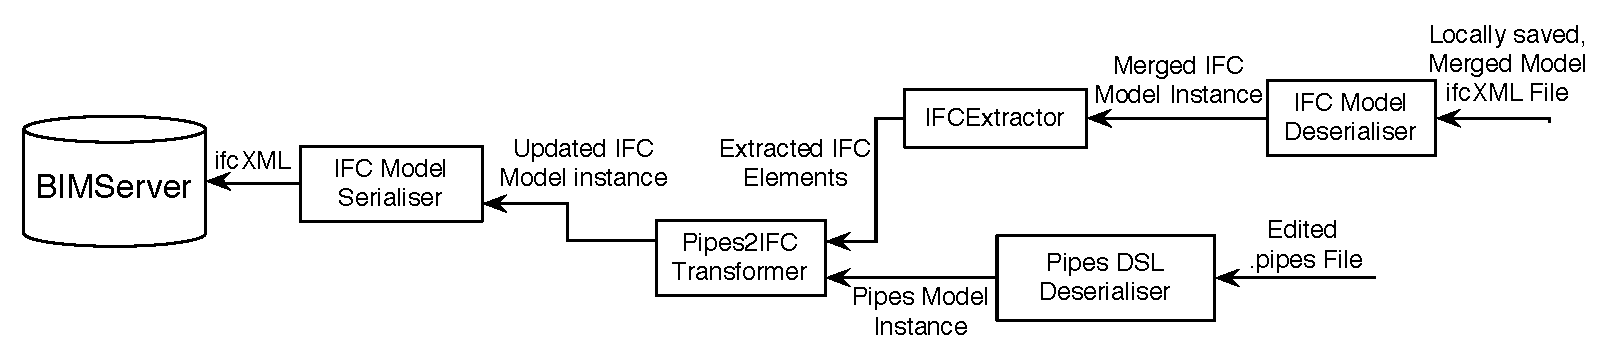
\includegraphics[width=120mm]{images/Pipes2IFC.pdf}
    \caption{Pipes2IFC workflow. Updates the main IFC model with the changes written in the Pipes DSL editor, then sends the IFC model back to BIMServer.}
    \label{fig:Pipes2IFCWorkflow}
\end{figure}
\subsubsection{Pipes2IFC}
Figure \ref{fig:Pipes2IFCWorkflow} shows the second workflow. As MWE2 workflows run in their own processes, it is necessary to deserialise the IFC model again, this time using the cached ifcXML. Consequently, the IFCExtractor must also be invoked again to get an instance of the extracted model. The Pipes2IFCTransformer will then compare the extracted model with an instance of the edited Pipes DSL, and update the IFC model with the result. To determine if an element has been added, updated, or removed, Pipes2IFCTransformer will check global IDs in the following way:
\begin{itemize}
\item If a global ID appears on an element in the Pipes DSL model, which does not exist in the IFC model, the element is transformed to its IFC equivalent, and added to the IFC model.
\item If a global ID exists in both models, but the elements have different metadata, the IFC element is updated.
\item If a global ID exists in the IFC model, but not in the Pipes DSL model, it is removed from the IFC model.
\end{itemize}
When the IFC model has been appropriately updated, a simple cleanup routine removes any orphaned elements or references, and the model is serialised as ifcXML. The ifcXML is then sent to BIMServer as a new revision.
 %Describe the solution
%!TEX root = ./report.tex
\section{Evaluation}
\label{sec:evaluation}
In this section we evaluate the solution, with reference to each of the requirements in Section \ref{subsec:requirements}. Furthermore, we discuss the methods used to verify the correctness of the prototype.

% Maybe: Discussion of applicability of product. What should be done in order to make this project usable in a real world scenario?

\subsection{Requirements Evaluation}
\label{subsec:requirements_evaluation}
\subsubsection{R1. Working with a Partial Model}
We are capable of extracting partial IFC models, and subsequently updating these by using the Pipes DSL editor. In Section \ref{subsec:problem_analysis} we presented the informal definition of the IFC subset that we extract, and in Figure \ref{fig:pipes_dsl_ecore_model} we depicted the corresponding Pipes DSL meta model. We focus on a simple partial model, but it would be possible to extend this if other IFC objects were to be added. We have ensured modularity by implementing the extraction process as a modular workflow component. Hence, the extraction process is verifiable as confirmed by the automated tests described in Section \ref{subsec:verification_methods}.

\subsubsection{R2. Correct Meta Model} As explained in Section \ref{subsec:ifc_meta_model}, the prototype uses the official ifcXML XSD to generate an Ecore meta model that is both correct and replaceable, in theory. However, there are certain serious drawbacks to this solution.

EMF does not seem to handle the large IFC meta model very well. The IFC meta model generated from the ifcXML XSD, was incomplete, with certain methods not being generated (eUnset methods for fields in some entity classes). Also, EMF generated methods that exceeded the maximum size allowed by the Java Development Kit (64kB)\footnote{JDK bug 4262078: \url{http://bugs.sun.com/view_bug.do?bug_id=4262078}}. While it is possible to work around such problems, it is not viable that the generated code has to be corrected.

One of the desirable features provided by using the generated meta model, was the availability of serialisers in EMF. However, these turned out to be too slow for working with realistic IFC models. A real-world model can easily result in load and save times of more than ten minutes. The EMF site lists some performance tips that should solve these problems\footnote{EMF Performance Tips: \url{http://www.eclipse.org/modeling/emf/docs/performance/EMFPerformanceTips.html}}\footnote{Performance and Extensibility with EMF: \url{http://www.slideshare.net/kenn.hussey/performance-and-extensibility-with-emf}}, but the improvement was minimal, if any. Thus, all of our tests have been carried out using smaller subsets of IFC models. 

\subsubsection{R3. Valid Model Transformations} 
To validate our transformations, both automated white box tests and black box test are used. The testing methods are described in detail in Section \ref{subsec:verification_methods}, and the results can be found in Appendices \ref{app:blackboxtests} and \ref{app:automatedtests}.

\subsubsection{R4. A Simple DSL} Section \ref{subsec:pipes_dsl} describes the benefits of the DSL implementation. It serves as a proof of concept that other subdomains of IFC can be edited in the same way. Being a modular component of the entire prototype, the textual Pipes DSL editor could be substituted with a visual one.

\subsubsection{R5. Structural Editing}
The prototype supports the addition and removal of both flow segments and openings, and thus the requirement is fulfilled.

\subsection{Verification Methods}
\label{subsec:verification_methods}
We have implemented automated test workflows for verifying that our transformation components work as desired. The IFCExtractor, IFC2PipesTransformer, and Pipes2IFCTransformer components (see Figure \ref{fig:Pipes2IFCWorkflow}) are the most interesting to validate, as these are the central components containing most of the transformation logic. Furthermore, black box tests of the entire prototype have been conducted with four input test buildings. These tests check that both the IFC model and the Pipes model is left in a valid state after running each workflow component. The results of the tests can be found in Appendices \ref{app:blackboxtests} and \ref{app:automatedtests}.

\subsection{Threats to validity}
\subsubsection{Internal Validity} When a prototype is primarily black box tested, it is natural to question the correctness of all the individual components. However, we argue that it is highly likely that any internal errors, undiscoverable by the black box tests, will either be discovered by the automated tests or result in program crashes, as the workflow components are highly modular with well-defined interfaces raising error flags if invalid input is provided.

Using EMF we have encountered a substantial amount of technical difficulties related only to the Eclipse IDE and its modelling tools. We identify these tools as an internal threat to the validity of the prototype, as our trust in them has been decreasing over the course of the project.

\subsubsection{External Validity} Retrieving building models for testing has been challenging. Given the fact that most modern visual BIM tools are very complex, we were unable to produce meaningful construction and plumbing models for testing, and had to rely on external contacts for providing test models (see Section \ref{sec:conclusion}). That means four example models were used for testing, which is considered sufficient, but not optimal. More tests with more example models must be performed to solidify the claim of general applicability of the prototype to all building models.








%!TEX root = ./report.tex

\section{Ideas for Future Projects}
\label{sec:plan_for_future_projects}
An overall goal of this pilot study is to increase the BIM knowledge of the environmentally concerned ITU research initiative, Energy Futures. With this project as a point of departure, we have developed the following ideas for future follow-up projects.

\subsection{Tools for Custom Open Source IFC Meta Model}
At the core of the prototype described in this paper, is the IFC meta model. As described in Section \ref{subsec:requirements_evaluation}, our meta model generated from the ifcXML XSD has several problems, such as the lack of inverse relationships. Most of these problems could be solved by using a better, customised Ecore meta model, such as one made by Steel. However, using this meta model would require writing serialisers, which is not a trivial task. With Steel's Ecore meta model as a starting point, one could imagine an open source project in which a full-fledged serialiser and deserialiser for the IFC-EXPRESS format is developed, along with a revision of the IFC meta model. This would enable developers to benefit from an independent, open source toolset for working with IFC in EMF, making them less dependent on proprietary tools.

% Study these papers:
%	"Feature-Based Survey of Model Transformation Approaches",
%	"The View Update Problem for XML",
%	"From model transformation to incremental bidirectional model synchronization" (very technical paper)
\subsection{Synchronisation}
If BIM client software is to be useful in a real world scenario when working on a partial model, it should be able to synchronise with the central model. As it was outside the scope of this project to require this kind of synchronisation for concurrent editing scenarios, our prototype is rather static compared to what is desirable for a final product. To be able to approach the synchronisation problem, we believe it is possible to expand on the current transformations implemented with Xtend. The addition of tracing would make it possible to track which transformation rules are applied to which elements in the source and target models, thus making it easier to verify the correctness of the transformations. For this purpose, Xtend offers a tracing package.\footnote{Xtend tracing package: \url{http://download.eclipse.org/modeling/m2t/xpand/javadoc/1.2/org/eclipse/xtend/util/stdlib/tracing/package-summary.html}} A project on synchronisation could investigate how a simple domain like Pipes DSL can handle proper synchronisation with a source model, possibly using BIMServer.

\subsection{Structural Changes}
Handling structural changes in the source model is challenging. With Pipes DSL, we simply insert new elements without taking changes in the source model into account, which is too na\"{i}ve to work in real-world scenarios. For example, when inserting a new pipe, an existing cost or energy object in the building model might need to reference this newly inserted object. We have allowed this type of constraint to be broken by our prototype, as it is not clear how dependencies and constraints should be checked. We believe that domain specific software, capable of defining constraints for the IFC model and automatically validating it, would be useful. The project would require a clear definition of the target domain and a study of relevant real-world models.






%!TEX root = ./report.tex
\section{Related Work}
\label{sec:related_work}
The problem of partial model editing and synchronisation is a common one. Here, we present a couple of closely related projects as well as other important alternative approaches and resources.

%A Graphical User Interface for Handling IFC Partial Model exchange
Nour argues that the exchange of partial models is one of the central challenges of widespread use of a central model for BIM, mainly IFC\,\cite{nour08}. Although we do not adopt his idea of end-user filtering through the use of MVD, our approach does incorporate software filtering for defining a working subset of IFC.

%BSPro COM-Server -- interoperability between software tools using industrial foundation classes
Karola et al. describe an early solution to the partial model extraction and update problem implemented as middleware. The BSPro COM-Server bridges various existing tools, each requiring a specific subset of IFC, making interoperability possible\,\cite{karola02}.

\hyphenation{To-ma-set-ti}
%Embedded Software Development with Projectional Language Workbenches
%PrEdE: a Projectional Editor for the Eclipse Modeling Framework
An alternative to our approach, is projectional editing. As specified by Tomasetti et al.\,\cite{tomasetti11}, projectional editors operate directly on the model, and thus no model synchronisation is involved. An example of a projectional editor is Jetbrains MPS.\footnote{Jetbrains MPS can be found at \url{http://www.jetbrains.com/mps/}} This approach trades loss of notational flexibility for a guarantee of model consistency\,\cite{conf/models/Voelter10}. Consequently, in order to bring the notation as close to the domain as possible, a projectional editor was not desirable for our solution.

%Towards a Framework for a Domain Specific Open Query Language for Building Information Models
Another way to derive and edit subsets of an IFC model is through the use of the BIM Query Language\,\cite{mazairac10}. This language provides access to IFC models via an SQL-like syntax. The queried model is stored on a BIMServer. While the BIM Query Language does provide much more flexibility in terms of extraction and editing of IFC data when compared to the prototype presented in this paper, it does not provide the same closeness to the chosen subdomain.

%From model transformation to incremental bidirectional model synchronization
%The View Update Problem for XML
Staworko et al. define and discuss the view-update problem for instances where both the view and the source are XML documents\,\cite{staworko10}. Any Ecore model, i.e. also the Pipes DSL model, can be converted to XMI, thus making the formalisations of both the view-update problem and its solutions are very relevant for the future work on our synchronisation logic.

%Feature-Based Survey of Model Transformation Approaches
The model transformations used in our prototype has mainly been realised through the direct manipulation approach described by Czarnecki et al.\,\cite{czarnecki06}, facilitated by the dispatch method feature of Xtend and the clarity of the MWE2.

As the design of the concrete syntax for the presented DSL has been a minor aspect of our prototype, it is far from perfect. The guidelines for DSL design presented by Karsai et al.\,\cite{karsai09} has been used as the basis for the preliminary design of the DSL, and further work in this direction will most likely benefit from the guidelines.




%!TEX root = ./report.tex
\section{Conclusion}
\label{sec:conclusion}
As evaluated in Section \ref{sec:evaluation}, the requirements for a partial editor prototype set forward in Section \ref{subsec:requirements}, have been met. Furthermore, the correctness of the output has been verified with an account for threats to validity. Specifically, we have\ldots

\begin{itemize}
\item Shown that it is feasible to define and edit a partial IFC model for a specific domain using a concrete syntax, the Pipes DSL.
\item Developed an editor for the Pipes DSL with syntax highlighting and autocompletion using Xtext. A comparison between the Pipes DSL syntax and the IFC-EXPRESS syntax was shown in Figure \ref{fig:pipes_express_comparison}.
\item Changed metadata and edited the structure of a building model using the Pipes DSL. To the extent that all our tests run as expected, we believe that these changes happen correctly.
\item Been able to interface with a BIMServer instance to store building models and merge a construction model and a plumbing model into a coherent IFC model used by the workflows shown in Figures \ref{fig:IFC2PipesWorkflow} and \ref{fig:Pipes2IFCWorkflow}.
\item Presented ideas for projects that can improve upon the prototype and evolve the area of open source BIM software.
\end{itemize}

We believe that through the exploration of how model-driven development can be used with IFC, this pilot study has provided a valuable starting point for further research in this area, which the ITU research initiative Energy Futures can build upon. In conclusion, we find that editing of a partial IFC model defined by a concrete, real-world domain is feasible using the model-driven methodology.

\subsubsection{Acknowledgements} Special thanks to associate professor at Aalborg University Kaj A. Jørgensen for providing example IFC models as well as overall guidance in selecting a fitting IFC domain for our project. Furthermore, we thank construction management student at Copenhagen School of Design and Technology, Mathias Demant for providing example IFC models mainly used for testing.
%!TEX root = ./report.tex
\bibliography{report}

%% Old bibliography
% %
% % ---- Bibliography ----
% %
% \begin{thebibliography}{99}
% %

% \bibitem[3]{2mich:tar}
% Michalek, R., Tarantello, G.:
% Subharmonic solutions with prescribed minimal
% period for nonautonomous Hamiltonian systems.
% J. Diff. Eq. 72, 28--55 (1988)

% \bibitem[4]{2tar}
% Tarantello, G.:
% Subharmonic solutions for Hamiltonian
% systems via a $\bbbz_{p}$ pseudoindex theory.
% Annali di Matematica Pura (to appear)

% \bibitem[5]{2rab}
% Rabinowitz, P.:
% On subharmonic solutions of a Hamiltonian system.
% Comm. Pure Appl. Math. 33, 609--633 (1980)


% \end{thebibliography}
%!TEX root = ./report.tex
\newpage
\appendix
\section{Results of Black Box Tests}
\label{app:blackboxtests}
\subsection{Input Models}
For these tests, we have several input models: One of them is a subset of a real IFC model, provided by Kaj Jørgensen. The rest of the test models have been created by Mathias Demant for our tests, and do not represent any real buildings. The files can be found in Prototype/Model2ModelWorkflows/NanoLabBuilding/ on the attached medium. The results can be seen in Figures \ref{fig:test1}, \ref{fig:test2}, \ref{fig:test3}, and \ref{fig:test4}.
\subsection{Tests}
For each case, we will perform the following tests between the two MWE2 workflows:
\subsubsection{Test 1:}
Modifying the metadata (name, description) for one of each of the three product types (wall, opening, flow segment).\newline\textbf{Expected result:} The output IFC model differs from the input IFC model in that it has altered metadata (name, description).
\subsubsection{Test 2:}
Modifying the placement of one of each of the three products types.\newline
\textbf{Expected result:} A new IFCLocalPlacement object now exists in the IFC output model with the modified metadata. 
\subsubsection{Test 3:}
Modifying the list of walls in a opening element.\newline
\textbf{Expected result:} A new IFCRelVoidElement is present in the output IFC model, compared to the input mode, linking the wall and opening.
\subsubsection{Test 4:}
Deleting a Pipe.\newline
\textbf{Expected result:} The output IFC model no longer contains the deleted flow segment. Any created orphans should be garbage collected.
\subsubsection{Test 5:}
Adding an Opening.\newline
\textbf{Expected result:} The output IFC model should now contain the created opening, along with any new objects referenced by the opening (LocalPlacement, Axis2Placement3d)
\subsubsection{Test 6:}
Adding one opening, deleting one flow segment, and modifying metadata for one wall.\newline
\textbf{Expected result:} The output IFC model should now contain the created opening (along with referenced objects), the flow segment should be deleted (along with orphans), and the metadata for the wall should be updated.
\begin{figure}
    \centering
        \centerline{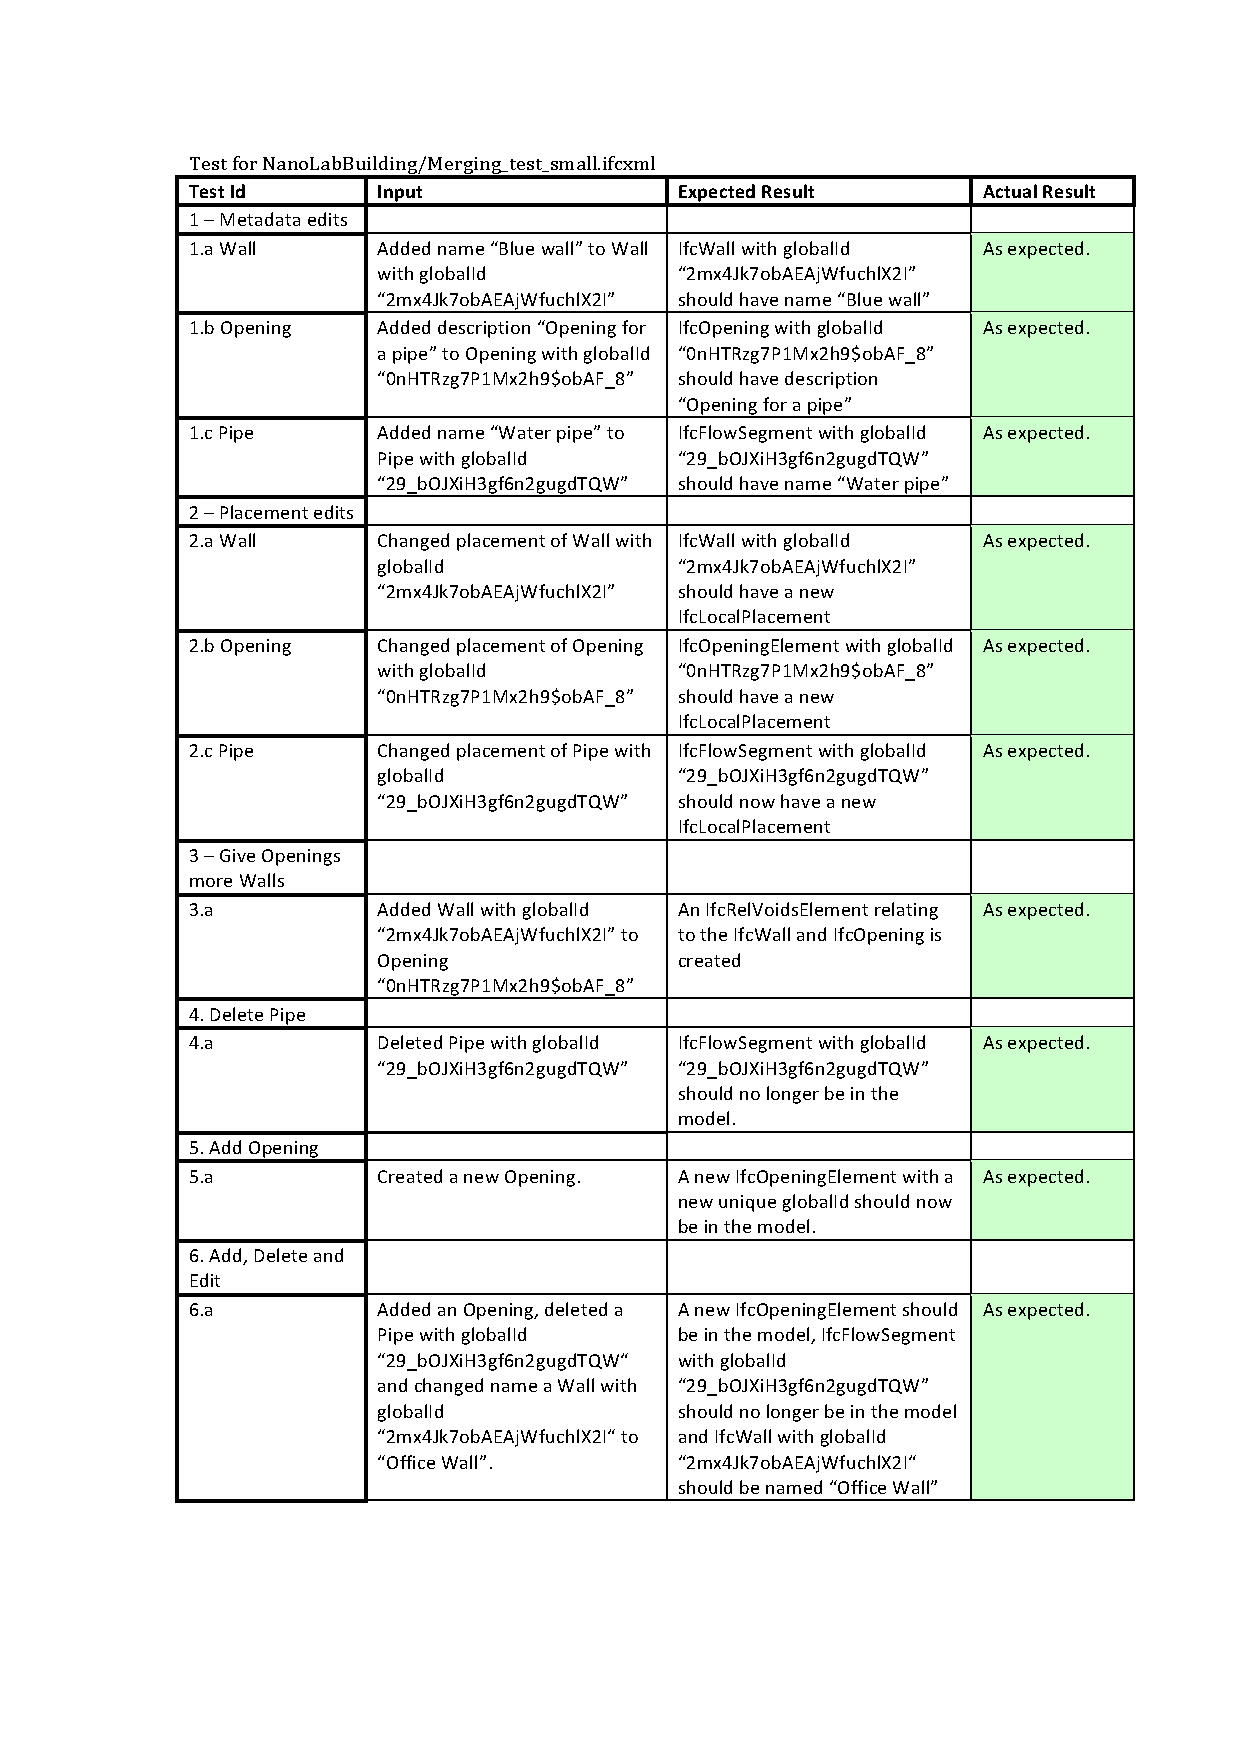
\includegraphics[width=150mm]{images/Test1.pdf}}
    \caption{}
    \label{fig:test1}
\end{figure}
\begin{figure}
    \centering
        \centerline{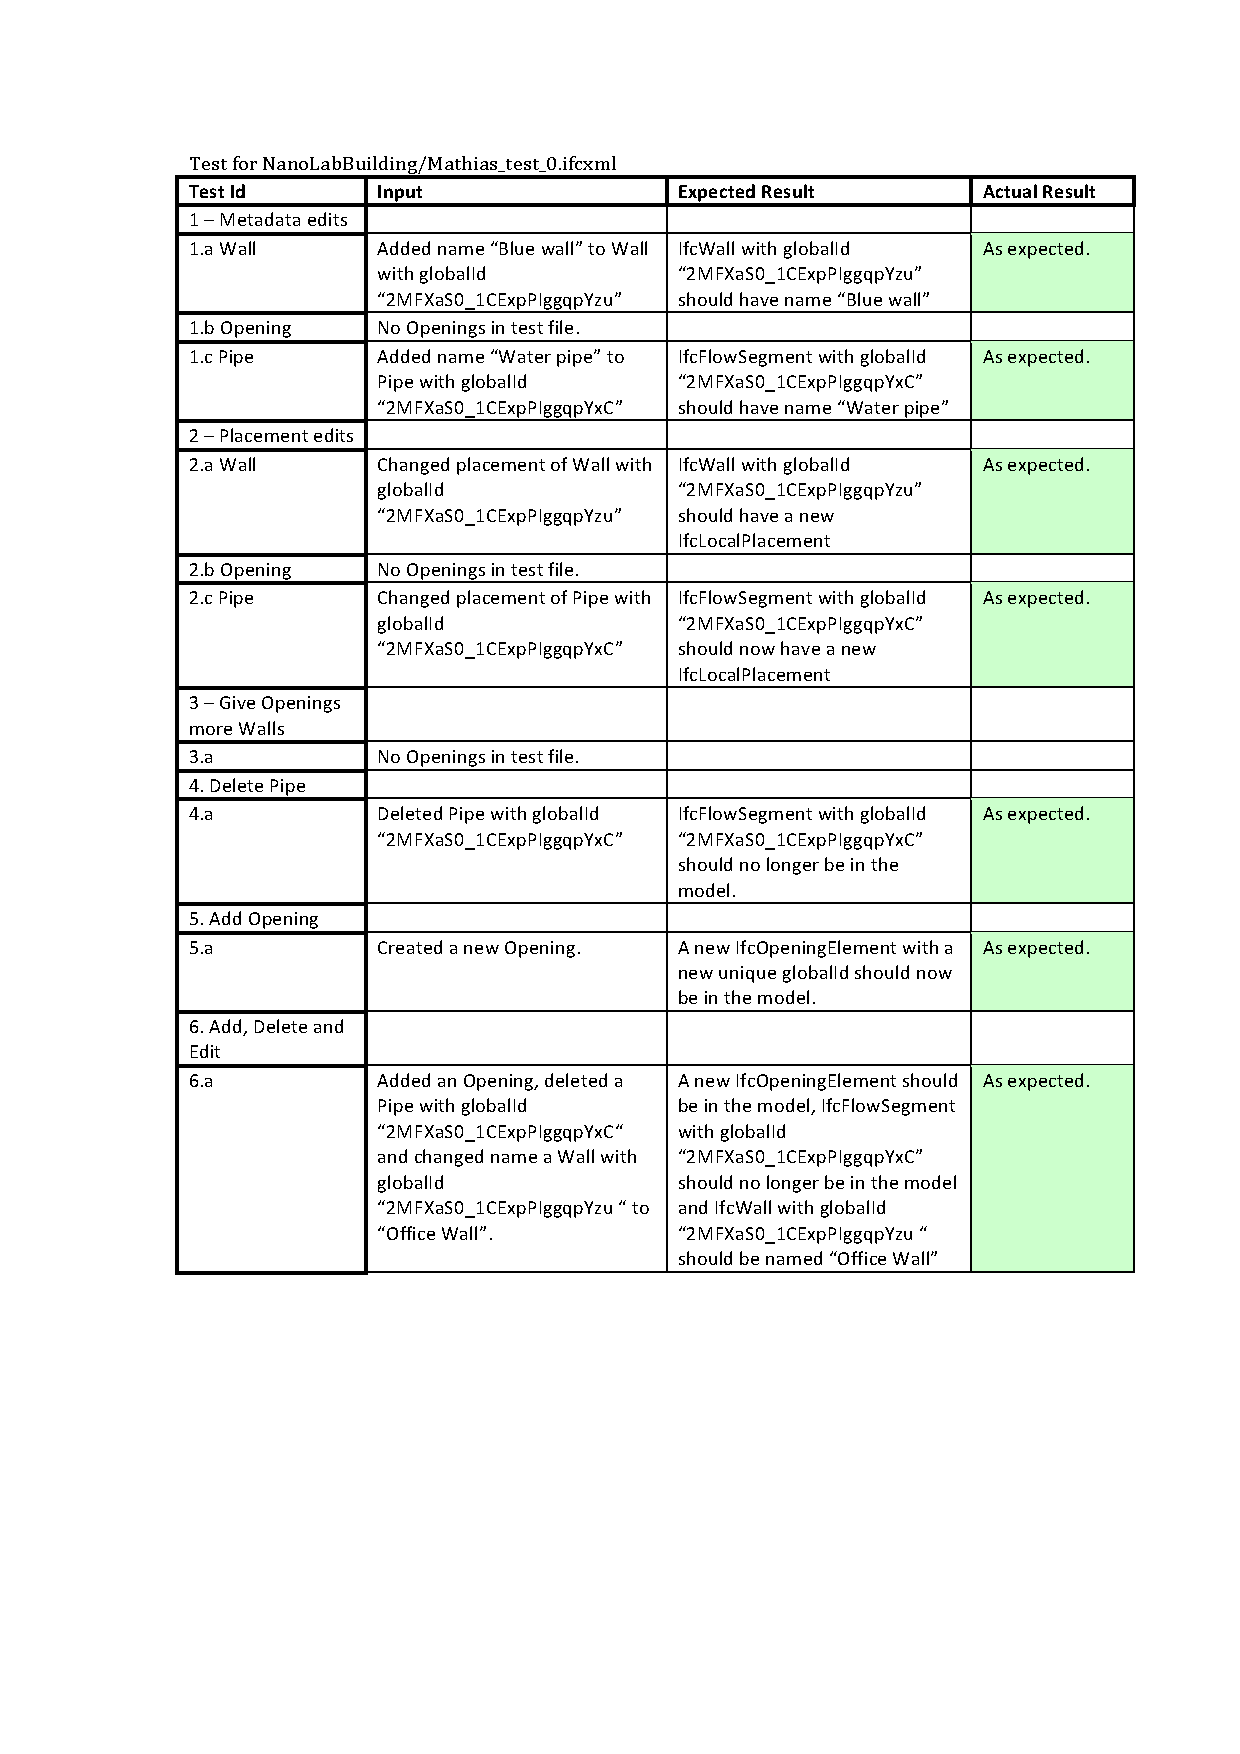
\includegraphics[width=150mm]{images/Test2.pdf}}
    \caption{}
    \label{fig:test2}
\end{figure}
\begin{figure}
    \centering
        \centerline{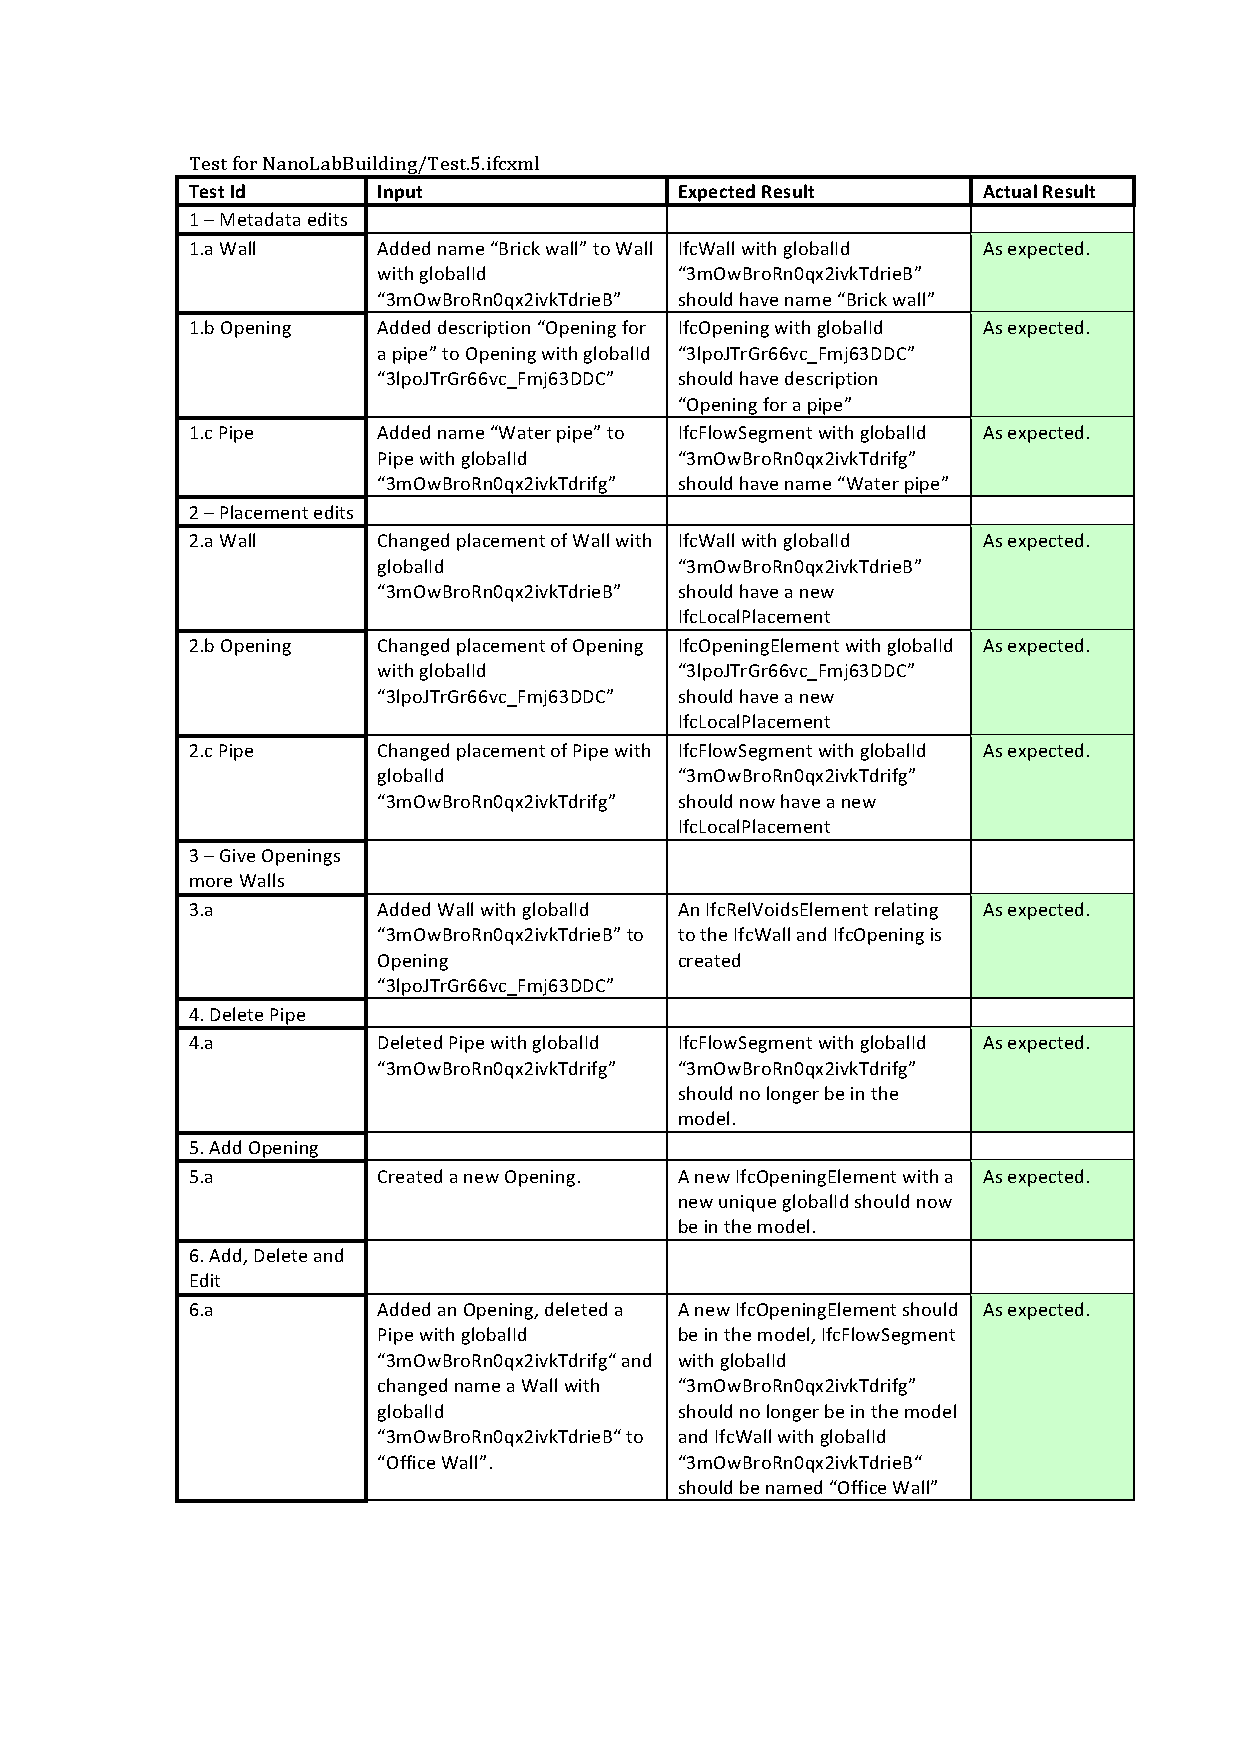
\includegraphics[width=150mm]{images/Test3.pdf}}
    \caption{}
    \label{fig:test3}
\end{figure}
\begin{figure}
    \centering
        \centerline{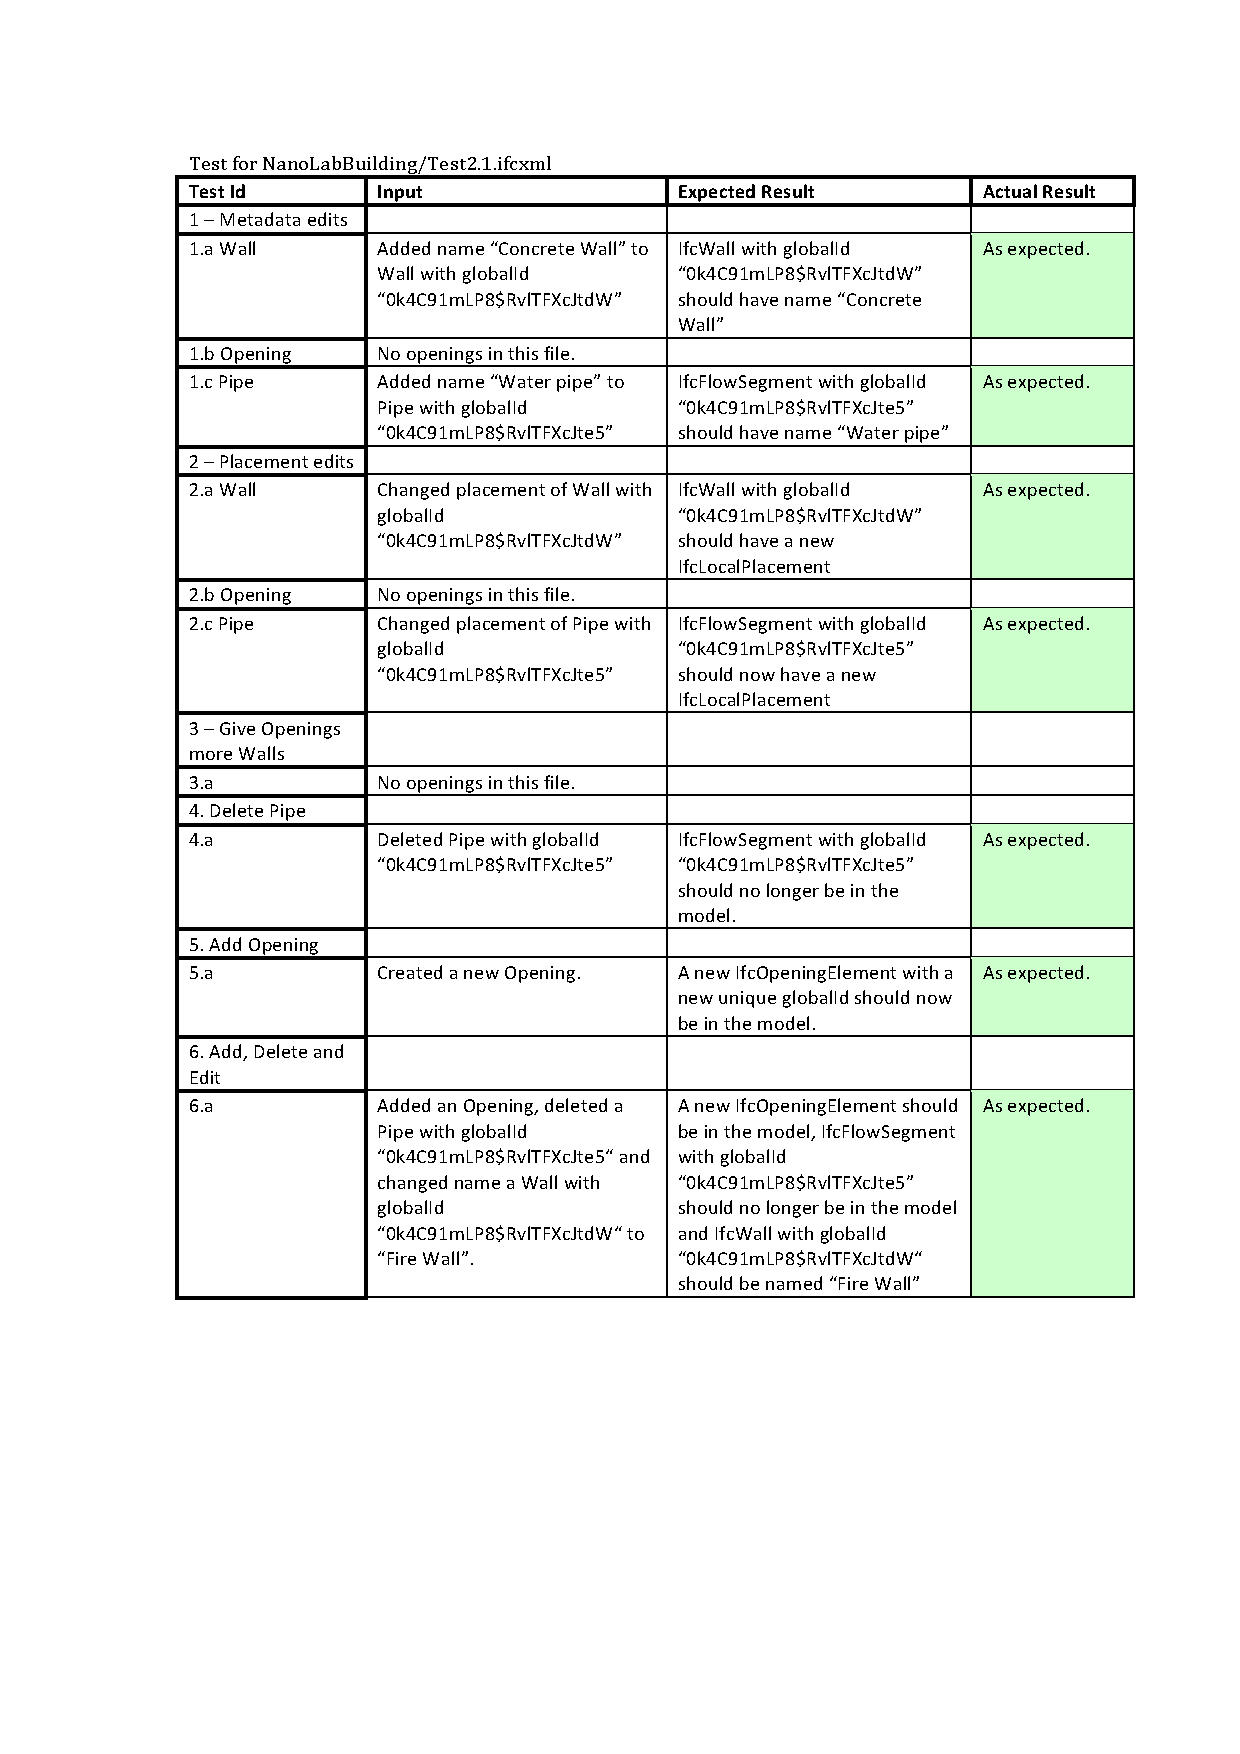
\includegraphics[width=150mm]{images/Test4.pdf}}
    \caption{}
    \label{fig:test4}
\end{figure}


\section{Automated Tests}
\label{app:automatedtests}
The workflow components used for tests can be found in the Eclipse project under: Model2ModelWorkflows/src/tests. These components work as a part of two test workflows similar to the ones used in the actual prototype. The only difference is that test components have been inserted after extraction and transformation components in the test workflow. The IFC2Pipes.mwe2 workflow is thus tested by the IFC2PipesTest.mwe2 workflow and the Pipes2IFC.mwe2 workflow is tested by the Pipes2IFCTest.mwe2 workflow.

\subsubsection{Testing Element Extraction}
The TestIFCExtractor workflow component verifies that the extraction process executed with a correct result. On any input building it checks that the number of extracted IfcProducts corresponds to the number of products that should be extracted by looking directly at the ifcXML. For each of the extracted product elements it tests for a valid globalId and Id. The tests have been run with the Merging\_{}test\_{}small model, only as this is the most realistic model. All assertions succeed in this test.

\subsubsection{Testing IFC to Pipes Model Transformation}
The following consistency verification between elements in the IFC and Pipes models are carried out:

\begin{itemize}
	\item IfcFlowSegment <-> FlowSegment
	\item IfcOpening <-> Opening
	\item IfcWall <-> Wall
	\item IfcLocalPlacement <-> LocalPlacement
	\item IfcAxis2Placement3d <-> Axis2Placement3D
	\item IfcDirection <-> Direction
\end{itemize}

By going through all extracted IFC products after the model to model transformation and comparing them to the elements of the Pipes model, the TestTransformers test component automates transformation testing of the subdomain. All consistency tests on Merging\_{}test\_{}small pass.

\subsubsection{Testing Pipes-to-IFC Update Routine}
The TestTransformer test component is used for the purpose of testing the Pipes-to-IFC update routine as well. The same consistency checks are performed after the Pipes2IFCTransformer, which executes the update routine. The same element relations as above are tested. All consistency tests on Merging\_{}test\_{}small pass.








\end{document}









